\documentclass{article}
\usepackage{graphicx}

\title{Ejercicio Paracaidista con Euler Explícito}
\author{}
\date{}

\begin{document}

\maketitle

\section{Ecuación diferencial}

La velocidad de caída de un paracaidista en función del tiempo viene dada por la siguiente ecuación:

\[
\frac{dv}{dt} = g - \frac{c}{m}v
\]

Siendo \( g \) la constante gravitacional, \( m \) la masa y \( c \) el coeficiente de arrastre.

\section{Análisis y dibujo}

Analizar ecuación (módulo) y dibujar los vectores principales del escenario. Incluir las condiciones iniciales (p.ej. una persona de 80 Kg de peso que saltó de una cabina a 36 Km de altura, dió un pequeño paso adelante, vel (1,0) m/s).

\section{Iteración con método de Euler}

Iterar con el método de Euler para ir obteniendo la velocidad en los 10 primeros segundos (\( dt = 1 \)).

\begin{table}[htbp]
    \centering
    \begin{tabular}{|c|c|}
    \hline
    \textbf{Parámetros} & \textbf{Ecuación diferencial (aceleración)} \\ \hline
    \( dt \) & 0.1 \\ \hline
    \( g \) & 9.8 \\ \hline
    \( m \) & 60 \\ \hline
    \( c \) (coef. arrastre) & 80 \\ \hline
    \end{tabular}
\end{table}

\section{Aceleración del paracaidista}

Para sacar la \textbf{aceleración} del paracaidista hay que tener en cuenta que

\[
\vec{a}_{paracaidista} = \frac{d\vec{v}}{dt} = \vec{g} - \frac{c}{m} \times \vec{v}
\]

\section{Velocidad de Euler}

Para sacar la \textbf{velocidad de Euler} se obtiene con

\[
\vec{v}_{i+1} = \vec{v}_i + \vec{a}_{i} \times dt
\]

\section{Velocidad analítica}

Para sacar la \textbf{velocidad analítica} se obtiene con

\[
v = \frac{gm}{c}(1 - e^{-(c/m)t})
\]

\section{Error de Euler}

Y para obtener el \textbf{Error de Euler} se hace el valor absoluto de la diferencia entre el resultado de Euler y el analítico.

\[
\left| v_{euler} - v_{analitica} \right|
\]

\begin{figure}[htbp]
    \centering
    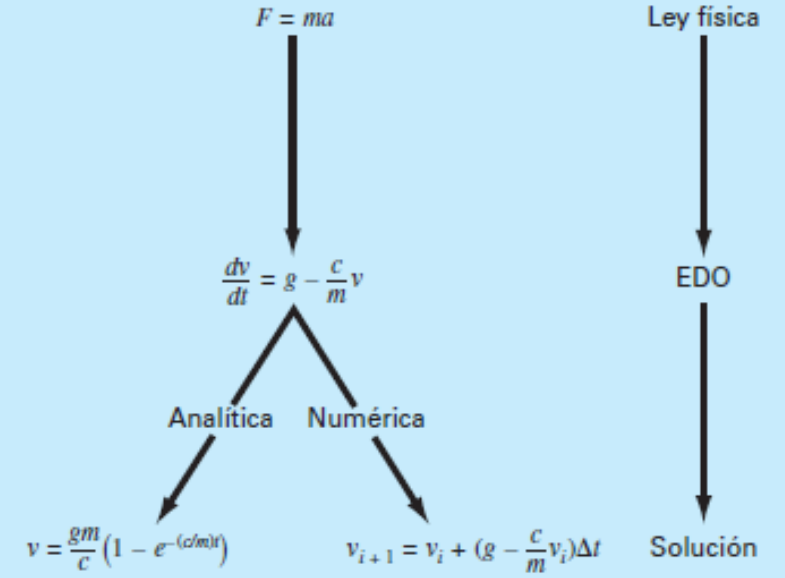
\includegraphics[width=0.5\textwidth]{AnaliticaNumerica.png}
    \caption{Gráfico de la solución analítica y numérica.}
\end{figure}
\newpage
\section{Resultados}

Los resultados en una tabla quedarían así:

\begin{table}[htbp]
    \centering
    \begin{tabular}{|c|c|c|c|c|}
    \hline
    \( t \) & \( A = \frac{dv}{dt} \) & \( V_{Euler} \) & \( V_{analitica} \) & Error(Euler\_exp) \\ \hline
    0,00 & 9,80 & 0,00 & 0,00 & 0,06 \\ \hline
    0,10 & 8,49 & 0,98 & 0,92 & 0,11 \\ \hline
    0,20 & 7,36 & 1,83 & 1,72 & 0,14 \\ \hline
    0,30 & 6,38 & 2,57 & 2,42 & 0,17 \\ \hline
    0,40 & 5,53 & 3,20 & 3,04 & 0,18 \\ \hline
    0,50 & 4,79 & 3,76 & 3,58 & 0,19 \\ \hline
    0,60 & 4,15 & 4,24 & 4,05 & 0,19 \\ \hline
    0,70 & 3,60 & 4,65 & 4,46 & 0,19 \\ \hline
    0,80 & 3,12 & 5,01 & 4,82 & 0,19 \\ \hline
    0,90 & 2,70 & 5,32 & 5,14 & 0,18 \\ \hline
    1,00 & 2,34 & 5,59 & 5,41 & 0,17 \\ \hline
    1,10 & 2,03 & 5,83 & 5,65 & 0,16 \\ \hline
    1,20 & 1,76 & 6,03 & 5,87 & 0,15 \\ \hline
    1,30 & 1,53 & 6,21 & 6,05 & 0,15 \\ \hline
    1,40 & 1,32 & 6,36 & 6,21 & 0,00 \\ \hline
    \end{tabular}
\end{table}

\begin{figure}[htbp]
    \centering
    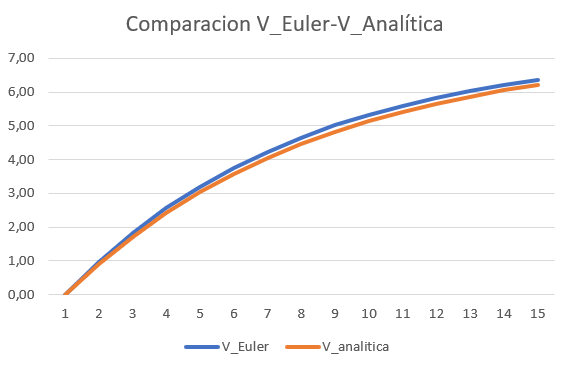
\includegraphics[width=0.5\textwidth]{EulerAnalitica.png}
    \caption{Comparación entre la solución numérica (Euler) y analítica.}
\end{figure}

\end{document}
